\documentclass[conference]{IEEEtran}
\IEEEoverridecommandlockouts
\usepackage{cite}
\usepackage{amsmath,amssymb,amsfonts}
\usepackage{algorithmic}
\usepackage{graphicx}
\usepackage{textcomp}
\usepackage{xcolor}
\def\BibTeX{{\rm B\kern-.05em{\sc i\kern-.025em b}\kern-.08em
    T\kern-.1667em\lower.7ex\hbox{E}\kern-.125emX}}
\begin{document}

\title{Techniques to manage cache unpredictability in Real Time systems: A Survey\\}

\author{
    \IEEEauthorblockN{
        Ananay Sharma\IEEEauthorrefmark{1},
        Daman Bir Singh\IEEEauthorrefmark{2},
        Hemlatha Pandey\IEEEauthorrefmark{3}, and
        Tejal Karnavat\IEEEauthorrefmark{4}
        }
    \IEEEauthorblockA{
        ME Computer Science, BITS Pilani K K Birla Goa Campus, 2020\\
        \IEEEauthorrefmark{1}2020H1030072G
        \IEEEauthorrefmark{2}2020H1030065G,
        \IEEEauthorrefmark{3}2020H1030067G, and
        \IEEEauthorrefmark{4}2020H1030044G
    } 
}

\maketitle

\begin{abstract}
    In Real-Time Systems, for effective scheduling of hardware resources, all components must have a predictable performance.  Cache memories inherently have unpredictable access which can vary a lot during multiple runs of the same task. As a result they are not considered for Real Time Systems which is a substantial disadvantage when it comes to system performance. In this paper, we survey various solutions for improving the predictability of cache memory in Real Time Systems and their effect on performance.
\end{abstract}
\bigskip
\begin{IEEEkeywords}
    Real Time System, Cache Memory, Cache predictability,Memory hierarchy, Cache Design Architecture, Cache Partitioning, Re-configurable Cache
\end{IEEEkeywords}

\section{Introduction}
    The essence of a real time system lies in its ability to exhibit a correct logical behaviour and more importantly, reach that correct result within a fixed time restriction. Real time systems are often employed in sensitive environments where an error in the result or a delay in calculating the result would lead to destruction of capital and maybe even loss of human life. Such systems are termed as Hard Real Time systems which cannot afford to violate time constraints associated with the tasks. Therefore, real time systems must be precise and predictable. Predictability of a real time system acts as one of its core concepts which helps us to decide whether the system can satisfy the deadline of a task or not.\\
    Advancements in the field of semiconductor chips led to the development of multi-core processors. Multiple computing units on a single processor chip would mean parallel execution of instructions and therefore, an increased computing power. As a result, real time systems that demanded more computing power than the past uniprocessor setup emerged. Multi-core platforms were also more cost effective than uniprocessor systems in terms of performance per cost. However, multi-core setups introduced new challenges associated with the predictability of a real time system.\\
    The ability of a real time system to perform a task within a certain time limit is proved through a schedulability analysis\cite{b8}. A basic assumption, common to all such analysis techniques, is that the upper bound of the worst case execution time(WCET) of each task in the real time system is known. Now, this calculation of WCET is especially difficult in multi-core architectures due to resource sharing among cores. Unchecked contention of shared resources among the cores introduces unpredictability at run-time. Execution of a task at a core would be subject to availability of a specific resource(s) at a particular instance of time during run-time. Cache memory is one such shared resource. Arguably, cache memory experiences the most frequent interactions with the cores of a processor among all shared resources.\\
    Cache memory exhibits incredible memory access performance in a general purpose system but they introduce this unpredictability which is highly undesirable for a real time system. Cache memory is used to bridge the gap between the high speed of the processor and relatively slower speed of the main memory. In modern multi-core setups there are typically two to three levels of cache between the core and the main memory. Generally, level-1(L1) cache is private to each core in the processor. Consecutive levels, level-2(L2) and/or level-3(L3) cache may be shared between all cores or a particular cluster of cores in the processor. The last level of cache(LLC) right before the main memory is shared by all the cores. This type of hierarchy relies on spatial and temporal locality of memory access to reduce execution time because cache miss has the highest impact in increasing execution time of a task.\\
    Two types of cache behaviour is identified\cite{b7}:
    \begin{itemize}
        \item \textbf{Intrinsic behaviour}: it is independent of the execution environment and depends only on the limitations provided by the hardware(e.g. number of cache lines available or the size of memory available) and the program code. Cache misses due to this behaviour can be reliably predicted by a static analysis, because the configuration of the system is fixed in hardware and the code of the task that will run on it.
        \item \textbf{Extrinsic behaviour}: It is dependent on the execution environment of the given task. This includes the pre-emptive scheduling within the system. Hence, cache misses occuring due to this type of behaviour cannot be reliably predicted because assumptions of locality of memory access(for the pre-empted task which will be rescheduled) may or may not be violated as a result of pre-emption.
    \end{itemize}
    Depending on the behaviour of cache hierarchy, certain interferences are introduced which affect the execution time of a real time task:
    \begin{itemize}
        \item  \textbf{Intra-task Interference}\\
        Intra-task interference occurs when tasks have their working set sizes greater than a specific cache level. This means that two memory entries in a working set are mapped in the same cache set. As a consequence the task is forced to evict its own cache lines. First, the initial required data is loaded into the cache, then it needs more data to finish execution, so it removes the initial data from the cache line and loads the new required data. This results in increased execution time. Intra-task interference also occurs in single core systems.
        \item \textbf{Intra-core Interference}\\
         Intra-core happens within one core. Specifically, when a pre-empting task removes a pre-empted task's cached data for execution, then the pre-empted task will have to load its data back into the cache whenever it is rescheduled resulting in increased execution time of the pre-empted task. The delay of data access in this case will be dependent on the cache replacement policy which is implemented in the system.
         \item \textbf{Inter-core Interference}\\
         Inter-core interference occurs mainly in multi-core setups. It occurs when tasks running on different cores concurrently access a shared level of cache. If the two tasks map to the same cache line, they can evict each other repeatedly in the cache and introduce unpredictability of execution time of both tasks.\\
    \end{itemize}
 
    Deriving the worst case execution time of a task within a real time system is an important aspect of validation of the system. Computing WCET tests whether the system meets the time constraints or not. Broadly there are two approaches to estimate the upper bound on WCET. First method is the static analysis wherein the binary code of the task is analysed without execution using certain estimation tools which compute the WCET. Static approach is highly pessimistic to account for the real scenario and highly unreliable for complex multi-core architectures. The second method uses experimental measurement where binary code of the task is executed on hardware multiple times, and WCET is then extracted from the results with a certain confidence figure and is further inflated with 20 to 30 percent error margin to account for possible unobserved  instances. This experimental approach however, might lead to overestimation.\\
    These derivation techniques however, become complex with use of caches because execution time of an instruction may vary depending upon:
    \begin{itemize}
        \item The location of data/instruction in the memory hierarchy.
        \item Cache Hit/Miss.
        \item Cache coherence protocol used in case of shared cache systems.
        \item Cache replacement policy used.
    \end{itemize}
     
     Due to this behaviour, static analysis methods have strict limits when it comes to shared cache systems as they cannot account for above factors before run-time. Even after computing WCET, inter-core interference complicates the validation of a real time system. Unregulated access of shared cache memory in a multi-core setup makes it difficult to achieve temporal isolation. Management of cache memory in a multi-core system is therefore essential for achieving a reliable real time system.

\section{Survey of Protocols}

\subsection{\textbf{The use of cache memory in Real Time Systems\cite{b1}}}

    M.K.J. Milligan and H.G. Cragon in their paper proposed a system to improve the upper limit of cache’s execution time by modifying the distribution of Inter Miss Distance (IMD). IMD is the distance between two successive cache misses as shown in figure \ref{fig_a_1}.
    
    \begin{figure}[htbp]
        \centerline{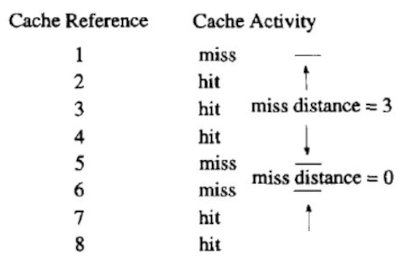
\includegraphics{Inter_Miss_Distance.JPG}}
        \caption{Inter Miss Distance\cite{b1}}
        \label{fig_a_1}
    \end{figure}
    It was found that $t_{ea}$ which is the effective memory-access time and IMD are inversely proportional. In order to decrease the $t_{ea}$ to enhance overall system performance, design goals were set to maximize the IMD worst case. The two programs used for evaluating the cache design performance were SHUTTLE.c and LRCpr1.c.\\
    Initial simulations were made on modifying primary cache parameters like – cache size, cache type (unified/split), block size and associativity. Secondary parameters included replacement policies, write and copy back etc.
    \begin{figure}[htbp]
        \centerline{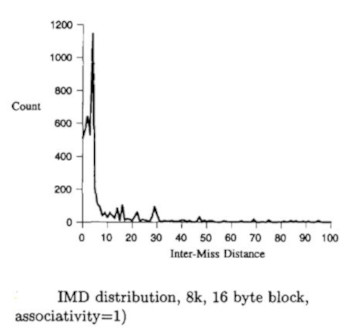
\includegraphics{IMD_Distribution.JPG}}
        \caption{IMD Distribution\cite{b1}}
        \label{fig_a_2}
    \end{figure}
    For a typical run the IMD distribution is given in figure \ref{fig_a_2}. From this it was determined that specific instances of IMD values can be eliminated by following certain design goals:
    \begin{itemize}
        \item Cache size $\geqslant$ 32k bytes
        \item Block size $\geqslant$ 256 bytes
        \item Especially for direct mapping (associativity = 1) split cache performs better than unified caches.
        \item Multi-way cache associativity performs better with unified cache.
    \end{itemize}

    Developing a pre-fetch architecture for anticipating cache misses was further proposed to improve cache predictability for real time systems.
    
\subsection{\textbf{Practical OS-Level Cache Management in Multi-Core Real-Time Systems\cite{b2}}}
    Hyoseung Kim et al.\cite{b2} have presented the idea of software cache partitioning to solve the problem of cache interference to use the shared cache in a predictable manner. Page coloring has been chosen as an approach which prevents interference from other tasks by allocating explicit cache partitions to each task while requiring no extra hardware support.
    But there are problems that need to be addressed:\\
    \begin{itemize}
        \item First, the memory co-partitioning. Along with cache memory is also partitioned which means if a certain number of cache partitions are allocated to a task, the same number of memory partitions also have to. This creates a problem when a task requires more or less memory.
        \item Second, availability of limited number of cache partitions. With an increasing number of tasks, the amount of cache available for each task gets reduced.
    \end{itemize}
    The proposed OS-level cache management scheme provides a way for predictable cache performance while getting rid of the aforementioned issues with the help of Cache reservation, Cache Sharing and Cache Aware Task Allocation. Cache reservation makes sure of exclusive use of cache while mitigating the inter-core cache interference. Inside a core, with cache sharing tasks can share the reserved cache while having a safe-upper bound on intra-core cache interference.\\
    The proposed OS-level cache management scheme provides a way for predictable cache performance while getting rid of the aforementioned issues with the help of Cache reservation, Cache Sharing and Cache Aware Task Allocation. Cache reservation makes sure of exclusive use of cache while mitigating the inter-core cache interference. Inside a core with cache sharing, tasks can share the reserved cache while having a safe-upper bound on intra-core cache interference.\\
    \begin{figure}[htbp]
        \centerline{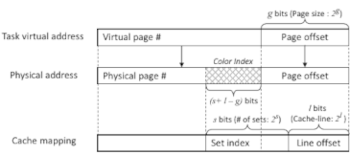
\includegraphics{Page_coloring.png}}
        \caption{Memory to cache mapping and page coloring\cite{b2}}
        \label{fig_b_1}
    \end{figure}
    The main concept in page coloring technique is in the mapping between cache entries and physical address, Fig. \ref{fig_b_1} is an example of how a cache entry is mapped to task’s memory address. Here,\\
    ‘g’  least significant bits refer to offset to a page.\\
    $2^l$  bytes per cache line\\
    $2^s$  cache sets\\
    ‘l’ bits are used as cache line offset.\\
    As, we can see, there is overlapping between bit physical page number and cache set index. These intersection bits are used as color index in Page Coloring technique which partitions the cache in $2^{(s+l-g)}$ partitions. It also co-partitions the entire physical memory into the same memory partitions. As the OS controls the mapping between virtual and physical memory address, a specific cache partition can be allocated by assigning a corresponding color memory partition.
    \begin{figure}[htbp]
        \centerline{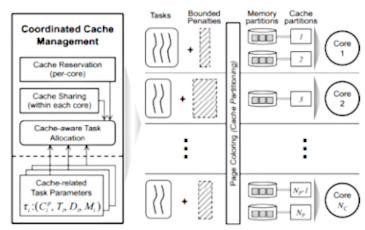
\includegraphics{Overview_cache_management.png}}
        \caption{Overview of the proposed OS-level cache management.\cite{b2}}
        \label{fig_b_2}
    \end{figure}
    We can see the overview for the scheme in Fig. \ref{fig_b_2} consisting of three components:
    \begin{itemize}
        \item Cache Reservation\\
        It ensures that each core gets exclusive use shared cache portion. But due to difficulties in accurately calculating inter-core interference in a multi-core machine, a portion of cache partitions is reserved for every core. These partitions are exclusively used by their owner cores.Within a core, the cache partition can be shared by multiple tasks thereby allowing more tasks than the number of cache partitions. This significantly reduces the waste of cache and memory due to the co-partitioning problem.
    \item Cache Sharing\\
    The  scheme allows sharing partitions for tasks running on same core, but causes intra-core cache interference. Cache partitions are allocated such that schedulability is preserved
    and memory requirements are guaranteed. There are two conditions for a cache allocation to
    be feasible.\\
    The first condition is the response time test, and the factors that affect a task’s response time
    are: 
    \begin{itemize}
        \item Cache-related task execution time.
        \item Cache partition refill time.
        \item The number of other tasks sharing the task’s cache partitions.
        \item The periods of the tasks sharing the cache partitions.
    \end{itemize}
    The second condition is for the task memory requirements.A  necessary and sufficient condition for cache sharing is: 
    For each cache partition $\rho$, the following condition must be satisfied:\\
    \newline
    $\sum_{\forall \tau_i : \rho \in S(i)} M_i/|S(i)| \leqslant M_{total}/N_p$\\\\
    where $M_i$ is the size of the memory requirement of $\tau_i$,\\
    $|S(i)|$ is the number of cache partitions assigned to $\tau_i$,\\
    $M_{total}/N_P$ is the size of a memory partition, and\\
    $M_i/|S(i)|$ represents $\tau_i$’s per memory-partition memory usage. \\
    This condition ensures that the sum of the per-memory-partition for the tasks sharing the cache partition $\rho$ should not exceed the size of one memory partition.
    \item Cache Aware task Allocation\\
    Cache Aware Task Allocation is an algorithm with the benefits of both cache reservation and cache sharing while allocating task and cache partitions. It aims to reduce the number of cache partitions required to schedule a given task set on a specified number of cores, so that other cores can be used for other purposes.
    According to the scheme, tasks assigned to the same core may share cache partitions. Therefore to take advantage of cache sharing, we should pack tasks into the same core as much as possible. So our algorithm is based on Best-Fit decreasing bin-packing algorithm, resulting in load concentration.
    \end{itemize}
    
\subsection{\textbf{Dynamic way-based cache partitioning and time-triggered scheduling with a reconfigurable cache\cite{b3}}}
    Gang Chen and others\cite{b3} presented a system with dynamic way-based cache
    partitioning at hardware level and a reconfigurable cache component. The schedule-aware  cache partitioning was done at the task-level. At compilation time, a number of cache configurations and a completely deterministic time-triggered non-preemptive schedule were generated. The framework used a share-clock multi-port timer and a customized reconfigurable cache component in order to create (multi-processor system-on-chip)MPSoCs with varying number of cores and different cache configurations by modifying the cache size, associativity and cache lines. These cache parameters were constituted at compile time whereas the cache partitions were reconfigured dynamically at run time. To avoid cache interference, cache ways were dynamically partitioned and allocated to tasks, thereby ensuring spatial isolation of cache. Also, the cores dynamically selected the cache ways as shown in the figure \ref{fig_c_1}, core 2 could select the 2nd and 5th way by using the cache configuration APIs.

    \begin{figure}[htbp]
        \centerline{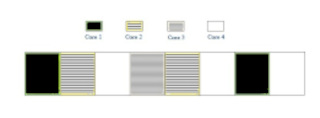
\includegraphics{CacheWayPartitioning_1.jpg}}
        \caption{Way-based Cache Partitioning.\cite{b3}}
        \label{fig_c_1}
    \end{figure}

    The proposed framework consisted of a synthesis approach for scheduling and cache management.The cache hierarchy of the system consisted of L1 caches for individual cores and a L2 cache, which was shared among the cores. The input specifications of the system contained three parts, namely, platform specification, map specification and task specification. The input parameters such as the number of cores, cache size, line size and associativity of the L2 cache came under the platform specifications. The task specification defined the timing requirements of the task, that is, the period and deadline, task profile information which included the WCETs(worst case execution time) of the tasks and cache miss number for variable cache sizes. To determine the worst case execution time, a measurement-based WCET estimation technique was used.
    
    The following notations were used for the system considerations:\\
    \newline
    $\tau = \{ T_1,  T_2, ….., T_n \}$, set of independent periodic tasks\break
    \newline
    $w_{ij}$ = WCET of task Ti $\in \tau$ with j ways of cache allocated to the task\break
    \newline
    $W_i = \{ w_{i1}, w_{i2}, ……, w_{iu} \} $,  WCET profile of task $T_i$, where u – total number of ways in the shared L2 cache\break
    \newline
    R $–$ set of all task profiles\\
    \newline
    $r_i \in R, r_i = <W_i, s_i, h_i, d_i>$, where,
    $s_i$ – start time, $h_i$ – period, $d_i$ – deadline, $W_i$ – WCET profile of task $T_i$, the deadline $d_i$ of the task $T_i$ was considered equal to its period $h_i$.\\
    \newline
    The relation between all the cores in the platform specification and all the tasks in the task specification was given by the mapping specification. The synthesis approach generated cache configuration and time-triggered scheduling for each task based on the input specification in such a way that the total cache miss number was reduced. It modeled the scheduling and cache interference using some timing and cache management constraints, which avoided cache overflow and missing deadlines, in turn, fulfilling real-time requirements. For a task Ti with profile $<W_i, s_i, h_i, d_i>$, the mth instance of task Ti starts at time instance, $s_i + m*h_i$. The WCET of a task Ti was given by $W_i$; a binary variable, $c_{ij}$ was used to denote the number of ways of cache allocated to a task $T_i$, such that,\\
    $T_i: c_{ij} = 1$, if j ways of cache were allocated to task $T_i$ and 0.\\
    Otherwise,the actual WCET of a task $T_i$, was attained as\\
    $\sum_{j=1}^{u}c_{ij}w_{ij}$, where u is the total number of ways in the shared cache.\\
    Every task has to finish no later than its deadline. This deadline constraint was given by,\\
    $s_i + \sum_{k=1}^{u} c_{ik}w_{ik} \leqslant d_i$
    
    
    The non-preemptive constraint was also defined to make sure that any two tasks mapped to the same core don’t overlap in time; that is, one must complete execution before the other one executes.
    The cache management constraints ensured that the sum of ways allocated to tasks running at any time instant should not go beyond the total capacity of the cache. To check for cache overflow, the lemma stated in \cite{b4}was used which is, “If the cache does not overflow at the start instant of
    any task within one hyper-period, the cache never overflows.” Thus, the  constraint was checked only at the time instant when any task started within one hyper-period.
    The reconfigurable shared cache, as shown in figure \ref{fig_c_2}, consisted of cache ways management unit(CWMU), cache control unit(CCU), core to Cache switch(CCS), and cache ways block(CWB). The cache ways were managed by the CWMU in a centralized way. Thus, cores could dynamically tune its ways by sending the reconfiguration command. The allocation and releasing of ways by the cores was centrally handled by the CWMU. The APIs used for cache reconfigurations such as allocation of ways, were atomic. The cache memory accesses were managed by the Cache Control Unit by instantiating N cache controllers for an N-core system. This enabled the cores to access cache concurrently. The cores were connected to cache ways dynamically by using the Core to cache switch(CCS). This was done by means of a ways mask register, maintained by the CWMU. For example, in figure \ref{fig_c_1}, core 2 can select the 2nd and 5th way by setting the ways mask as 0x48. To ensure well synchronized, precisely triggered tasks on different cores, a global timer was required to trigger all the cores in the system. For this purpose, a share-clock multi-port timer was used. The proposed framework incorporated time-triggered scheduling and cache partitioning so that the cache could be used predictably and effectively.
    
    \begin{figure}[htbp]
        \centerline{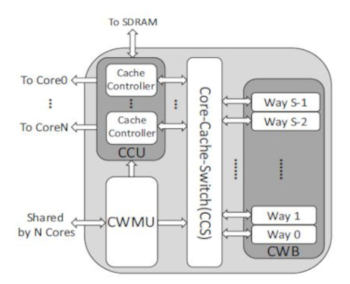
\includegraphics{ReconfigurableCache.jpg}}
        \caption{Reconfigurable Cache Architecture.\cite{b3}}
        \label{fig_c_2}
    \end{figure}

\subsection{\textbf{Criticality aware cache design\cite{b4}}}

    In [3], N G Chetan Kumar and others presented a cache design, which was criticality aware, for shared caches in mixed criticality real-time systems. It used a Least Critical(LC) cache replacement policy in order to reduce the response time of critical tasks. This policy targeted set associative shared caches by extending the conventional LRU(least recently used) cache replacement policy. A count of cache lines containing data from the critical address range (CAR) was maintained. Moreover, an LRU order for critical and non-critical lines present in each set of the cache was maintained. This order of either critical or non-critical lines was modified depending on the cache line being accessed during a cache hit. In case of a cache miss, the line to be replaced was selected according to the following order:
    \begin{itemize}
        \item Cache line, which is available
        \item Non-critical cache line, which was least recently used. 
        \item Critical cache line, which was least recently used, when all the lines present in a cache set were critical. The LC successfully degraded to LRU when all the lines in the cache were critical.
    \end{itemize}
    The figure \ref{fig_d_1} shows a working example of the LC cache replacement policy.
    \begin{figure}[htbp]
        \centerline{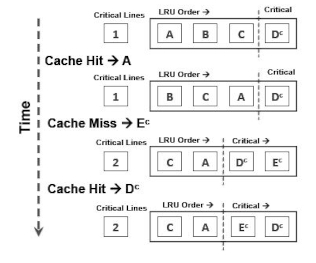
\includegraphics{LCexample.jpg}}
        \caption{Least Critical Cache Controller Block Diagram.\cite{b4}}
        \label{fig_d_1}
    \end{figure}

    The LC cache architecture contained four main components:
    \begin{itemize}
        \item Critical Address Range(CAR) compare: CAR registers were used to indicate where critical data resided in memory. These registers were used to identify critical cache lines while accessing the cache.
        \item Access History: The LRU order of critical and non-critical lines and the number of critical lines was maintained and updated with every cache access. A track of the number of cache lines in each cache set was kept.
        \item Tag Compare: The requested memory address was compared with tag bits associated with every cache line and accordingly, a hit/miss signal was generated.
        \item Data Control: An interface to the CPU for reading or writing data from/to the cache or main memory was provided.
    \end{itemize}
    The following figure shows a high level block diagram of the LC cache controller.
    \begin{figure}[htbp]
        \centerline{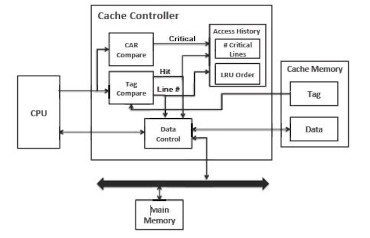
\includegraphics{LCblockDiag.jpg}}
        \caption{Least Critical Cache replacement policy working example.\cite{b4}}
        \label{fig_d_2}
    \end{figure}


\subsection{\textbf{Instruction cache in hard real-time systems: modeling and integration in scheduling analysis tools with AADL}\cite{b5}}
    Hai Nam Tran et al. (2014)\cite{b5} presented a model-based approach to boost the performance of cache in real time systems by reducing extrinsic interference which focuses on measuring the impact of Cache related preemption delay (CRPD). Integration of cache modeling and analysis methodology was made by using the scheduling analysis tool Cheddar and AADL (Architecture Analysis and Design Language) modeling language.
    As shown in figure \ref{fig_e_1} and figure \ref{fig_e_2}, initially the targeted system was modeled using AADL and then the cache analysis method was applied to real-time scheduling tool Cheddar. Finally, scheduling simulations were performed to examine the impact of CRPD.\\
    \begin{figure}[htbp]
        \centerline{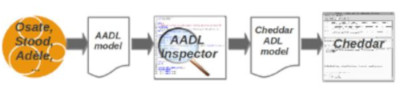
\includegraphics{Cheddar and analysis toolchain .JPG}}
        \caption{Cheddar and analysis toolchain.\cite{b5}}
        \label{fig_e_1}
    \end{figure}\\
    It was proposed that Cheddar which is an existing scheduling tool for real-time systems could be updated to include caches.\\
    \begin{figure}[htbp]
        \centerline{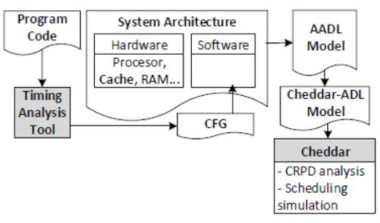
\includegraphics{Analysis Flow .JPG}}
        \caption{Analysis Flow.\cite{b5}}
        \label{fig_e_2}
    \end{figure}\\
    With AADL memory component, cache can be modeled but it doesn’t have all attributes. So some new attributes were proposed to precisely model cache memory. After following all the modeling, analysis and simulation steps the CRPD and WCET of the task were compared. It was found that if the WCET of two tasks are similar then assigning higher priority to the task having greater CRPD can avoid it from pre-empting.\\
    The impact of CRPD can be reduced by optimizing memory-to-cache mapping. Thus tasks using a small proportion of cache should be placed near each other in main memory.

\section{Conclusions}
    The proposed method\cite{b1} yields an improvement of 1.8 times in the worst case execution time by the elimination of all cache misses at IMD = 0. Modifying cache parameters like cache size, type, associativity and block size shows dramatic impact on performance. However, while designing a hard real time system, the worst case is of a particular interest so all the occurrences of IMD = 0 or 1 should be eliminated. It was found that with the increase of block size, IMD = 1 did decrease but elimination of all IMD = 1 occurrences became more difficult. Cache performance is dynamic and depends upon the program to be executed, although the program being used in this research was similar to an embedded real time system. Hence the relationship established between IMD distribution and cache parameters stands valid.\\
    \newline
    The coordinated OS-level cache management\cite{b2} scheme provides predictable performance on multi core systems with shared cache across cores without requiring any hardware support. It uses page coloring while handling the two main concerns about it, memory co-partitioning and limited number of cache partitions while giving a noticeable utilization improvement.
    But a big problem with page coloring based methods is large overhead it requires to perform recoloring. This overhead, firstly prevents a frequent change of colors and secondly makes the color changes of tasks with execution time smaller than the page-change overhead, futile. This shortcoming can be handled by hardware level cache partitioning which although requires hardware support but makes the overhead negligible.\\
    \newline
    On the other hand, by using dynamic way-based cache partitioning\cite{b3}, cache ways are partitioned without constraints, thereby leading to efficient use of limited cache and also ensuring isolation of the cache resource which avoids cache interference. Due to the use of a deterministic time-triggered non-preemptive schedule, the number of cache misses are minimised without missing deadlines and preventing cache overflow. The cache partitioning, done at hardware level with a customized reconfigurable cache component is performed with minimal timing overhead. The whole unused ways of the shared cache can be turned off thereby saving static energy and proving to be beneficial for low-power design.The partitioning is done on task-level, therefore, depending on the requirement of the tasks at run-time, allocation of cache ways can be handled. Thus, the system helps to make use of the shared cache in a predictable and efficient manner. However, the system requires hardware support in order to incorporate the reconfigurable cache and share-clock multiport timer for time-triggered scheduling.\\
    \newline
    Non-preemptive scheduling eliminates cache-related preemption delays(CRPDs) thereby reducing the need for complex and pessimistic CRPD estimation methods. The system strictly implements non-preemptive scheduling. But, in some scenarios, preemptive scheduling may be required. Thus, for reduction of impact of cache related preemption delay the model proposed in [5] extends existing scheduling tools to include cache.  The scheduling policy used decides the actual execution time of a task and number of preemption. This changes the cumulative CRPDs. However, the CRPD produces reverse impact on scheduling policy in many ways like priority assignment and feasibility tests. By comparing WCET and CRPD  and optimizing memory-to-cache mapping, reduction of CRPD can be achieved.\\
    \newline
    The criticality-aware cache design\cite{b4} enables fine grained control over classifying task data by providing a mechanism to store critical data in separate address spaces. This improves utilization of the cache and a higher preference is given to critical task data, thus, overhead caused due to locking/unlocking the cache is eliminated. Also, the critical address ranges can be changed dynamically thereby improving the performance of cache. Experimental results show that the cache miss rate of a critical task is reduced by upto 70\% while using LC cache as compared to LRU cache. But, if the size of critical data is increased, performance deteriorates. Also, this system considers only data caches. It could be further extended to instruction caches and support could be provided for data with multiple criticality levels.\\
    We need to implement cache access techniques which integrate cache coherence protocol and support multiple levels of criticality.The various solutions proposed above are aimed at improving the predictability of cache memory in Real Time Systems. All of these can be used at certain point depending on the available resources, scheduling policy and type of real time tasks.

\begin{thebibliography}{00}
\bibitem{b1}  M.K.J. Milligan and H.G. Cragon,``THE USE OF CACHE MEMORY IN REAL-TIME SYSTEMS'.
\bibitem{b2} Hyoseung Kim, Arvind Kandhalu, Ragunathan (Raj) Rajkumar, ``A Coordinated Approach for Practical OS-Level Cache Management in Multi-Core Real-Time Systems'', 2013 25th Euromicro Conference on Real-Time Systems.
\bibitem{b3} Gang Chen, Biao Hu1, Kai Huang1, Alois Knoll1, Kai Huang, Di Liu, Todor Stefanov, ``Automatic Cache Partitioning and Time-triggered Scheduling for Real-time MPSoCs'', 2014 International Conference on ReConFigurable Computing and FPGAs.
\bibitem{b4} N G Chetan Kumar, Sudhanshu Vyas, Ron K. Cytron, Christopher D. Gill, Joseph Zambreno and Phillip H. Jones, ``Cache Design for Mixed Criticality Real-Time Systems''.
\bibitem{b5} Hai Nam Tran, Frank Singhoff, St´ephane Rubini, Jalil Boukhobza,``Instruction cache in hard real-time systems: modeling and integration in scheduling analysis tools with AAD'', 2014 12th IEEE International Conference on Embedded and Ubiquitous, Milan.
\bibitem{b6} Giovani Gracioli, Ahmed  Alhammad, Renato  Mancuso, Antônio Augusto Fröhlich, Rodolfo  Pellizzoni,``A Survey on cache Management Mechanisms for Real Time Embedded systems''.
\bibitem{b7} Swagato Basumallick and Kelvin Nilsen: ``Cache Issues in Real-Time Systems". Iowa State University(May 1994).
\bibitem{b8} Robert I. Davis and Alan Burns`A survey of hard-real time scheduling for multiprocessor systems". Comput. Surveys 43, 4, Article 35(Oct 2011).
\bibitem{b9}S. Basumallick and K. Nilsen. Cache issues in real-time systems. In ACM Workshop on Language, Compiler, and Tools for Real-Time Systems, 1994
\bibitem{b10} W. Lunniss, S. Altmeyer, C. Maiza, and R. I. Davis, “Integrating cache related pre-emption delay analysis into edf scheduling,” University of York, York, UK, Technical Report YCS-2012-478, 2012.
\bibitem{b11} P. Dissaux, O. Marc, S. Rubini, C. Fotsing, V. Gaudel, F. Singhoff, A. Plantec, V. Nguyen-Hong, and H. N. Tran, “The smart project: Multiagent scheduling simulation of real-time architectures,” Proceedings of the ERTS 2014 conference.
\bibitem{b12} Gang Chen, Kai Huang, Jia Huang, Alois Knoll ``Cache partitioning and scheduling for energy optimization of real-time mpsocs'', In ASAP, 2013.
\end{thebibliography}
\end{document}
